%!TEX root = ../Thesis.tex
\chapter{Relevant Background}
\label{chap:reletiveBackground}

Depth perception is the ability of the Human Visual System \index{HVS} to visualize the three dimensional world as well as measuring the distance of an object based on two dimensional images obtained from the eyes. Depth perception is imperative for performing basic everyday tasks such as avoiding obstacles without bumping into them or interacting with the world with relative ease. In animals (specially predators), it is critical to estimate the distance of a prey for an efficient attack. Depth sensation is the term used for animals as it is not known whether they sense the depth in the same way as humans do or not\cite{ wiki:depth_perception}.

% Figure for cues
\begin{figure}
\begin{tikzpicture}[grow'=right,level distance=1.75in,sibling distance=.15in]
\tikzset{edge from parent/.style = {thick, draw, edge from parent fork right},
         every tree node/.style  = {draw,minimum width=1in,text width=1.3in,align=center}}
\Tree
    [. {Depth Information}
	        [.{Monocular Cues}
	                [.{Motion Parallax } ]
	            	[.{Depth from Motion } ]
	            	[.{Kinetic Depth Effect } ]
	            	[.{Perspective } ]
	            	[.{Relative Size} ]
	            	[.{Familiar Size} ]
	            	[.{Absolute Size} ]
	            	[.{Ariel Perspective} ]
	            	[.{Accommodation} ]
	            	[.{Occlusion} ]
	            	[.{Curvilinear Perspective} ]
	            	[.{Texture Gradient} ]
	            	[.{Shading} ]
	            	[.{Defocus Blur} ]
	            	[.{Elevation} ]
	        ]
	        [.{Binocular Cues}
	                [.{Stereopsis } ]
		            [.{Convergence } ]
		            [.{Shadow Stereopsis} ]
	        ]
    ]
\end{tikzpicture}
\caption{HVS Depth Cues\label{fig:CueTree}}
\end{figure}

Human visual system \index{HVS} uses several monocular and binocular cues to determine the depth of objects in the view. These cues can be categorized into two categories i.e. cues extracted from a single image (Monocular Cues) and cues extracted from two images (Binocular cues)\cite{depthcues1}\cite{ wiki:depth_perception}. Figure \ref{fig:CueTree} gives an outlook of the depth cues used by the HVS. These cues are then dynamically weighted according to their robustness by the HVS in order to estimate a depth value for each object in the view \cite{CueFusion}(Write details of those cues in Appendix).


\section{Binocular vision, stereopsis and its limits}
% Limits of stereopsis and that other paper of bank.\cite{banks1}
% cormack paper.
% when fusion and happens and when not and why?
Generally speaking, all the animals with two eyes have binocular vision and they can integrate the information from two eyes based on the binocular overlap. But the term Binocular vision is usually used for the animals that have a large area of binocular overlap (Human and most other predators) and use it to get the depth information of the world around them. In addition to calculating depth, binocular vision also has advantages in performing other tasks such as detection, discrimination, detecting camouflaged objects or eye-hand coordination. Even the resolution observed world is increased with binocular vision\cite{howard1995binocular}. Among all the depth cues discussed in the section above, Stereopsis is the most influential of them all. Since the human eyes are located at different lateral positions on the head, the images formed on the retinas of these two eyes are slightly different. The difference is mainly the horizontal positions of the objects\cite{ wiki:stereopsis}. The process of obtaining a fused (Binocular fusion) image (Cyclopean image) and obtaining a depth map based on the horizontal disparities of the objects in these two images is known as stereopsis.

When the eyes verge in order to focus on some object (or point) in space, that object is projected at identical corresponding points in the retinas. It means that the difference between their horizontal positions is zero. This process is called fixation of the eyes and the distance of the object (point) at which the eyes are fixated is called the fixation distance. The locus of all the points in space that is projected on identical retinal points is called the horoptor\cite{ wiki:horoptor}. Theoretically, via geometrical principles, the horoptor is a circular segment in the plane of fixation point. However, Wheatstone in 1938 observed that the actual/emperical horopter is much larger than that. Figure \ref{fig:horoptor} shows both the theoretical and empirical horoptor. Any object that is farther away from the horoptor has uncrossed disparity in the retinas i.e. the eyes need to be diverged (uncrossed) in order to fixate on that object. Similarly, any object that is closer than the horoptor has crossed disparity in the retinas i.e. the eyes need to be converged (further crossed) in order to fixate at it \textcolor{red}{cite and make the diagram for crossed uncrossed disparities}. Figure ?? shows a graphical representation of crossed and uncrossed disparities \textcolor{red}{add the dolphin images from wikipedia article.}.

\begin{figure}
\centering
    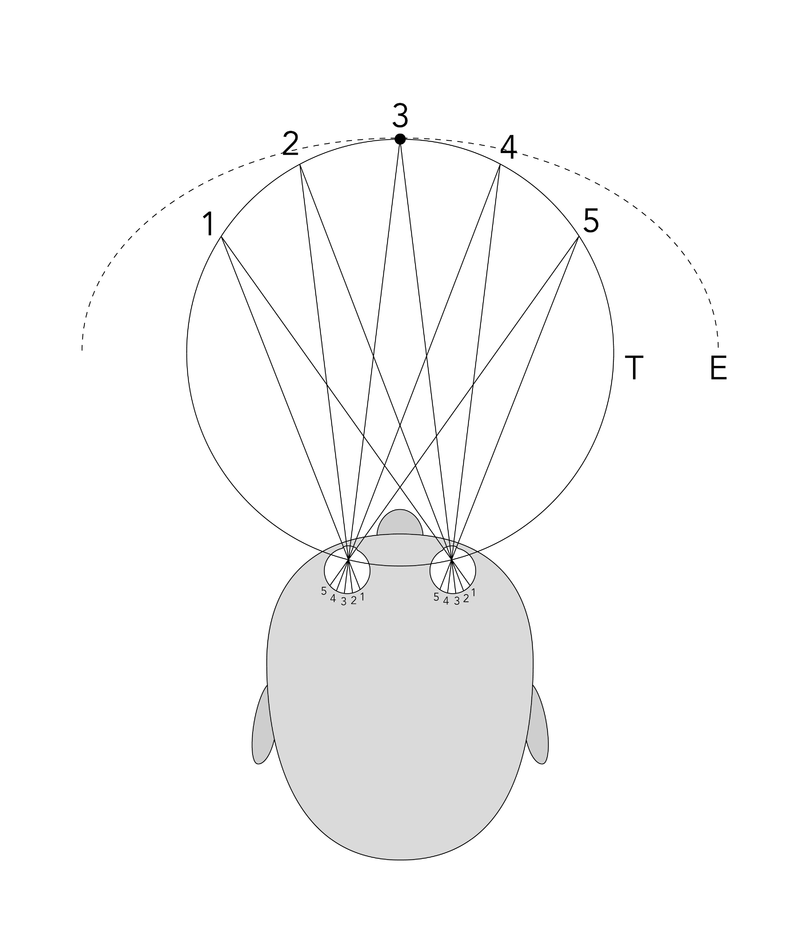
\includegraphics[width=0.5\textwidth]{./Template_Figures/horopter}
    \caption{Representation of theoretical (T) and empirical (E) horoptor\label{fig:horoptor}}
\end{figure}

Stereopsis is believed to be processed in the binocular neurons of the visual cortex of mammals. The binocular neurons have receptive fields in different horizontal positions in each eye. These cells are active only when the object of interest is in certain range of disparity in one eye relative to the other i.e. there is a maximum disparity limit. \textcolor{red}{add the dolphin images from wikipedia article.}. As the objects in the images formed at the retinas of both eyes are slightly shifted horizontally, presenting two different images with shifted object two both eyes can fool the HVS into perceiving depth. This process is called stereoscopy. The first stereoscope was invented by Sir Charles Wheatstone in 1838\cite{ wiki:wheatstone}. It used two mirror both tilted at 45 degrees to the eyes that reflected two different images from the sides. Currently all the stereoscopic screen present a different perspective image two both eyes with different technologies that will be discussed in later sections.

\section{Limits of Stereopsis}
% Limits of stereopsis and that other paper of bank.\cite{banks1}
% cormack paper.
% when fusion and happens and when not and why?
Put it in the section above.








\section{Crosstalk}
% Definitions and Factors contributing to Crosstalk
% Effects on viewers
% 70\% thing etc.
As discussed in the previous section, stereoscopy includes the process of displaying different perspective images to each eye in order to mimic the effect of depth in a scene. However, it is critical that the perspective of these two images should be segregated completely from each other. Currently, all the commercially available 3D displays (with exception of head mounted displays or Wheatstone setups) fail to isolate the two images completely. That means that a percentage of the image of one eye leaks to the other eye as well. This unintended leakage is called the crosstalk in stereoscopic screens\cite{woods2012crosstalk}. Figure \ref{fig:ct1} Shows one such example where the screen has a simulated crosstalk of 14\%. This means that 14\% image intensity of the right eye image is leaked into the left eye image and vice versa.

\begin{figure}[htbp]
    % \centering

    \begin{subfigure}[b]{0.3\textwidth}
        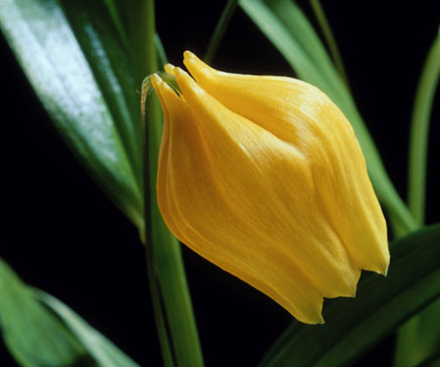
\includegraphics[width=\textwidth]{./Template_Figures/orig}
        \caption{Original Image}\label{fig:originalPicture}
    \end{subfigure}
    \begin{subfigure}[b]{0.3\textwidth}
        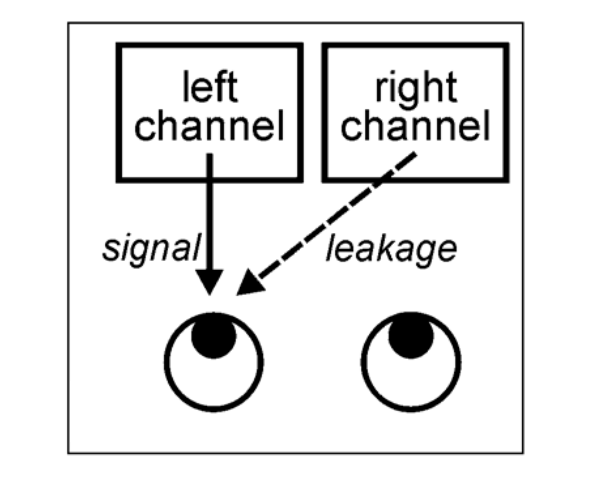
\includegraphics[width=\textwidth]{./Template_Figures/leakage}
        \caption{Original Image}\label{fig:ill_leackage}
    \end{subfigure}
    \begin{subfigure}[b]{0.3\textwidth}
        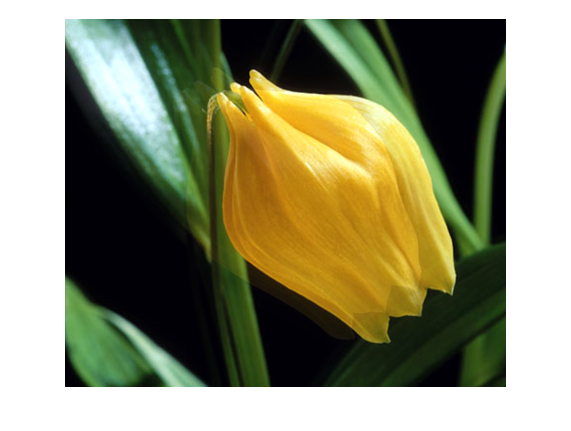
\includegraphics[width=\textwidth]{./Template_Figures/crosstalk}
        \caption{Original Image}\label{fig:imWCT}
    \end{subfigure}

    \begin{subfigure}[b]{0.3\textwidth}
        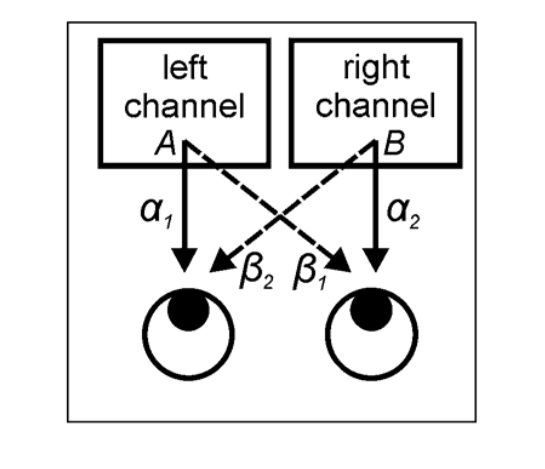
\includegraphics[width=\textwidth]{./Template_Figures/viewerCT}
        \caption{Viewers Crosstalk}\label{fig:viewerCT}
    \end{subfigure}

    \caption{(a-c) A simulation of 14\% crosstalk. An Image intended for the left eye containing 14\% of image intended for right eye. (d) Illustration of Viewers crosstalk with the transfer functions as defined by Andrew J. Woods \cite{woods2012crosstalk} \label{fig:ct1}}
\end{figure}

\say{System crosstalk} is the term used to define the amount of light leakage that occurs between two views and is independent of the image contents. In simplest form, it can be mathematically defined as:

\begin{equation}
Crosstalk(\%) = \frac{leakage}{signal} *100
\label{eq:simple_crosstalk}
\end{equation}

Here, \say{signal} is the luminance of the original image intended for an eye and \say{leakage} is the luminance of the light that leaks from the unintended image. Usually, on a stereoscopic scree, the amount of crosstalk is measured by observing the luminance of the left channel while a black (minimum luminance) image is displayed in the left channel and a white (maximum luminance) image is displayed on the right channel and vice versa. This definition is accurate for the screens that can manage to display a true black i.e. zero luminance. Almost all of the LCDs can not produce zero luminance as their minimum luminance hence resulting in a non-zero black level at its minimum. Another mathematical representation of crosstalk take into effect this non-zero black level and is defined as:

\begin{equation}
Crosstalk(\%) = \frac{leakage - black level}{signal - black level} *100
\label{eq:crosstalk_gray}
\end{equation}

Throughout the rest of the thesis, we will be using crosstalk as mentioned in eq \ref{eq:crosstalk_gray}.

Viewers crosstalk on the other hand is the amount of crosstalk that can be perceived by the viewer as ghosts. It is dependent on the image contents i.e the contrast at the ghosting point and the parallax of objects in the scene. If the system crosstalk is defined as
\begin{equation}
System\ Crosstalk\ (left\ eye) = \frac{\beta_2}{\alpha_1}
\label{eq:system_ct}
\end{equation}

Where \(\alpha_1\) denotes the percentage part of the left-eye image at position (x,y) as observed by the left eye and \(\beta_2\) denotes the percentage amount of right eye image at the same location (x,y) leaked into the left eye. Then the viewers crosstalk is defined as

\begin{equation}
Viewers\ Crosstalk\ (left\ eye) = \frac{B\beta_2}{A\alpha_1}.
\end{equation}

where \say{A} is the luminance of that particular point in left-eye image and \say{B} is the luminance of that particular point in right-eye image (as described in Fig \ref{fig:viewerCT}). The Variables \(\alpha\) and \(\beta\) are characterizing the transfer functions from the displayed image to the observed image i.e. the amount of light reaching the eyes after being displayed on the screen and going through the glasses or any other medium that resides between the screen and the eyes. In most displays, crosstalk is an additive process and is roughly linear. This means that to simulate crosstalk, adding a desired amount of unintended image to an intended image should be sufficient. The simulation of crosstalk in our experiments was carried out in the same manner.

The perception of crosstalk obeys the Webber's law which means that leaked light will be greatly perceivable by the viewer on the dark image areas rather than bright areas. Also, the perceived crosstalk is Dependant upon the contrast of the image and the binocular parallax of the stimuli i.e. crosstalk perception will increase with increase in contrast or increase in binocular parallax\textcolor{red}{Maybe I need to show why?}. It is commonly believed that ghosting plays the most critical role in determining the image quality. Wilcox and Stewart \cite{wilcox2003determinants} observed that over 75\% of the observers in their experiments reported the ghosting to be the key feature that deteriorated the image quality. Apart from reduction of image quality, perceivable ghosting is also responsible for loss of depth, viewer's discomfort, reduction of sharpness and contrast, decreased fusion limits, and difficulty in fusion. As mentioned earlier, two objects can not be fused together if the angular separation between them is smaller than the disparity\cite{burt1980disparity}. In fact since the ghost and the stimulus lie in the same (x, y) position but at different depth, the angular separation becomes zero and the disparity gradient of the ghost and the stimulus becomes infinity. Hence both of them can not be fused together. In this case the more luminant object i.e. the stimulus will be fused while the ghosts will remain in diplopic state\textcolor{red}{add the image showing infinity DG and cite the source}. Crosstalk in still images is perceived to a larger extant than crosstalk in dynamic scenes (e.g. a movie). This means that motion of objects in a scene can mask the perception of crosstalk.

The stereoscopic literature provides a lot of advices for the acceptable and unacceptable crosstalk for the viewers. Woods\cite{woods2012crosstalk} points some of these advices as:
\begin{itemize}
	\item Crosstalk between 2\% to 6\% significantly affects the visual quality and increase the viewers discomfort.
	\item In order to produce accurate depth range between 40 arcmin, the crosstalk should be as low as 0.3\%.
	\item Crosstalk is visible even at 1\% to 2\%.
	\item 5\% of crosstalk is enough to induce discomfort.
	\item JND for crosstalk is 1\%.
	\item 2-4\% of crosstalk can significantly decrease the amount of perceived depth.
\end{itemize}

As one can observe, there is a variability in these guidelines. The reason for this variability might be because of the different setups and types of stimuli that were used by the researcher in their experiments. We observed that currently the literature is not quite thorough on how the depth perception is affected when it comes to different kinds of stimuli and relatively more complex scenes. Which is why we performed some experiments of our own to verify and expand the current knowledge in this area. This is also one of the main contributions of this thesis.

\section{Stereoscopic/Automultiscopic Screens and its cross-talk}

In this section we will review some of the stereo technologies and their associated crosstalk. The basic setup for a stereoscopic displays involves a display screen that has typically higher (above 120 Hz) refresh rate and a view separation mechanism. A high refresh rate is required so that images from two different view perspective can be displayed alternatively without the user realizing any glitches (after the views has been separately delivered to the eyes). Various Stereo display technologies are available in the market such as CRT, DLP, Plasma, PDP and LCD screen. Active/Passive 3D glasses or anaglyph glasses are generally used as view separation mechanisms. Figure \ref{fig:ctflow} illustrates that the crosstalk is induced by the display as well as the view separator.

\begin{figure}
\centering
    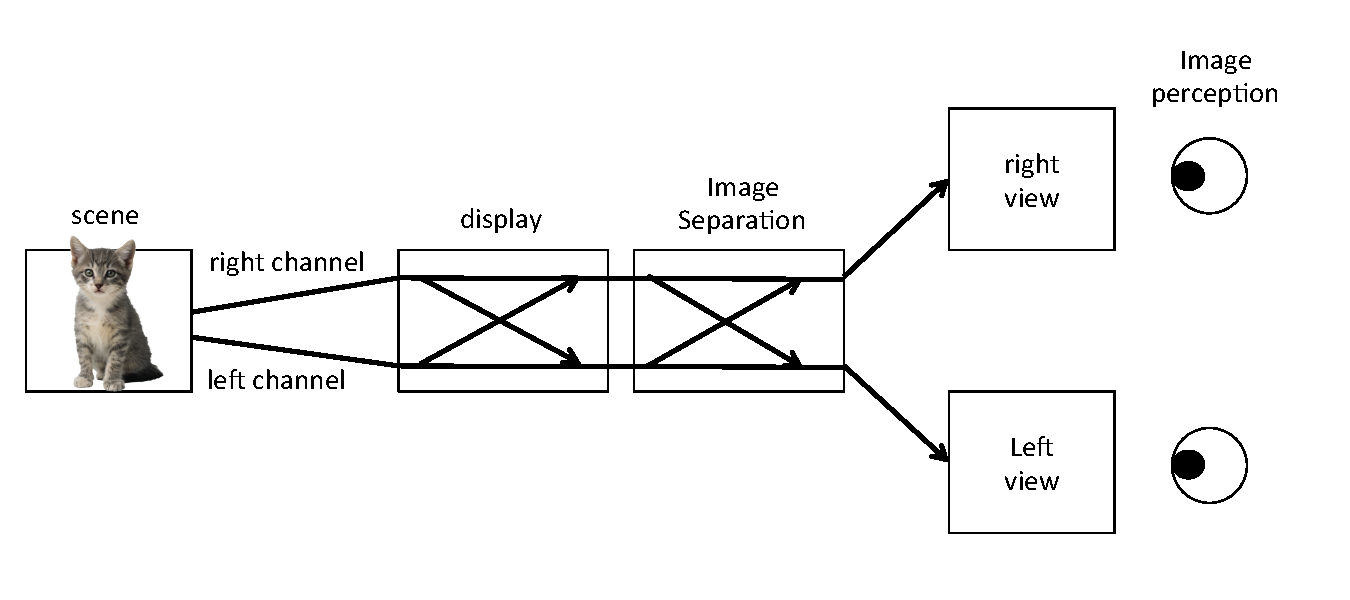
\includegraphics[width=0.9\textwidth]{./Template_Figures/ct_flow}
    \caption{A flow diagram showing the process of stereo image perception starting from stereo scene capture. The crosstalk can be induced by the display (light generation) and by the image/view separation mechanism(3D glasses or autostereoscopic parallax barrier).\label{fig:ctflow}}
\end{figure}

\subsection{Time sequential stereo using active shutter glasses with an LCD display}
LCD screen coupled with active shutter glasses is the most common 3D technology that is commercially available. It produces an image by back lighting a two dimensional individually addressable liquid crystal (LC) \index{LC}matrix. The back light is typically a cold cathode florescent lamp (CCFL) or light emitting diodes (LEDs). The LC matrix consists of crystals that rotate according to the voltage applied to them. This rotation limits the flow of the light that passes through each cell hence producing different gray levels. Each pixel of the screen consists of three LC cells coupled with red, green and a blue filter. Hence the color and luminance of each pixel is created by controlling the light that flows through these individual filters which is regulated by the LCs. It should be noted that even at its best i.e crystals are perpendicular to the light source, they fail to block the light completely and hence an LCD screen can not display true black color.

The time required for the LCs to rotate from one position to another desired position is known as the pixel response rate/time. This response time is higher if the delta between the rotate is smaller and vice versa\cite{woods2012crosstalk}. This means that the refresh rate of an LCD display is dependent upon this response time. LCD displays usually utilize top to bottom image update method i.e. in order to update the image being displayed, the rows of pixels is addressed individually from top to bottom.

\begin{figure}[htbp]
\centering
     \begin{subfigure}[b]{0.4\textwidth}
        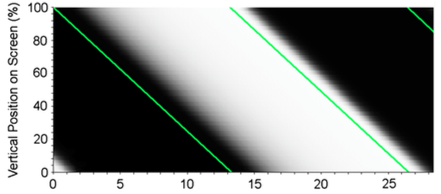
\includegraphics[width=\textwidth]{./Template_Figures/LCD_refresh_low}
        \caption{ Time(ms)}\label{fig:response_low}
    \end{subfigure}
    \begin{subfigure}[b]{0.4\textwidth}
        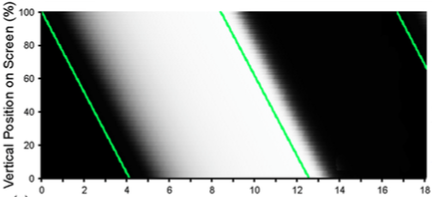
\includegraphics[width=\textwidth]{./Template_Figures/LCD_refresh_high}
        \caption{ Time(ms)}\label{fig:response_high}
    \end{subfigure}

    \caption{\textcolor{red}{(a) Response of a conventional LCD display (in time domain). (b) Response of a high refresh rate LCD display }.  \label{fig:LCD_refresh}}
\end{figure}

figure \ref{fig:LCD_refresh} shows the time domain responses of LCD displays. The green line represents the row of the pixels that are being updated while the images is being changed from complete black to complete white. It case be seen from \ref{fig:response_low} that there is no time (a vertical line) where a complete black or white image is observed. However if the refresh rate is increased (Figure \ref{fig:response_high}), one can see that there is an interval in time where a stable image can be displayed.

Active shutter glasses consists of lenses that can turn opaque or transparent in order to gate the left or right image being displayed on the screen to the respective left or right eye (at any given time, one lens is in opaque state while the other in transparent state). Each lens of these glasses has a liquid crystal called LC shutters(just like an LCD display) that blocks the light when a voltage is applied to it. The time required for these LCs to go from completely opaque to completely transparent and vice versa is called the rise and fall time \cite{woods2012crosstalk}. Figure \textcolor{red}{SHould I use the picture fig 4 from woods?} shows the optical transmission properties of a typical pair of active shutter glasses. It can be seen from this figure that
\begin{figure}
\end{figure}

\begin{itemize}
\item{LC shutters do not perform identically for each wavelength.}
\item{The LC shutters have a non zero transmission even when it is in opaque state.}
\item{The rise and fall time are not instantaneous.}
\end{itemize}

In addition to that, the light transmission in active shutter glasses also varies with the viewing angle. The highest blocking of the light occurs at an angle perpendicular to the shutters. This means that while viewing a scene through these shutter glasses, one would observe grater leakage of light in the border areas of the shutters as compared to the center (provided the position of the eye is in the center of the shutters). It is important that the shutters are opened and closed with the right timings with respect to the image being displayed on the screen. Incorrect image will be observed if the shutters are opened too early or too late that will result in crosstalk.

Hence, the methods according to which crosstalk can occur when using active shutter glasses combined with an LCD display are:
\begin{itemize}
	\item{Optical performance of the liquid crystal cells i.e. crosstalk is proportional to the amount of light leaked while in opaque state.}
	\item{Incorrect synchronization of shutter glasses with respect to the display.}
	\item{Viewing angle through the shutter glasses.}
	\item{Pixel response rate of the LCD display. Higher response time will result in higher crosstalk.}
	\item{Image update method. The ideal time for opening of a shutter would be when an image has been completely displayed on the screen. However most LCDs update the image using vertical scanning and hence usually there is no time at which the image is completely displayed stably.}
	\item{The x,y location of the image on the screen. This is related to both the image update method and the veiwing angle through the shutter glasses.}
	\item{The gray level being displayed. If the change in gray level is small then the response time will be large hence causing larger crosstalk. }
\end{itemize}

\subsection{Anaglyph Stereo}
\subsection{Active/Time Sequential Stereo on LCDs}
\subsection{Passive/ Space Multiplexed Stereo}
\subsection{Automultiscopic Screens}
discuss lightfeields here as well.

\section{Crosstalk Quality Metrics}